% 74-21(74쪽) — $y=a\sin\pi\left(x-\dfrac{1}{3}\right)+b$ 의 그래프(원문 「오른쪽 그림」). 스캔 화질이 낮아 TikZ 로 다시 그림.
% 라벨은 원문 것만: $3$, $-1$, $\pt{O}$, $c$, $\dfrac{5}{6}$(화살표), 그래프 이름. 원문에 없는 눈금은 적지 않는다.
\begin{tikzpicture}[line width=0.6pt, x=0.80cm, y=0.58cm, >=stealth]
  \draw[densely dashed, line width=0.35pt] (-0.95,3) -- (3.45,3);
  \draw[densely dashed, line width=0.35pt] (-0.95,-1) -- (3.45,-1);
  \draw[densely dashed, line width=0.35pt] (0.8333,0) -- (0.8333,3);
  \draw[densely dashed, line width=0.35pt] (1.8333,0) -- (1.8333,-1);
  \draw[->, line width=0.7pt] (-1.00,0) -- (3.60,0) node[below=1pt, font=\small] {$x$};
  \draw[->, line width=0.7pt] (0,-2.3) -- (0,4.0) node[left=1pt, font=\small] {$y$};
  \draw[domain=-0.85:3.30, samples=200, smooth] plot (\x, {2*sin(180*\x-60)+1});
  \node[anchor=east, font=\small, fill=white, inner sep=1pt] at (-0.04,3) {$3$};
  \node[anchor=north east, font=\small, fill=white, inner sep=1pt] at (-0.04,-1) {$-1$};
  \node[anchor=north east, font=\small, fill=white, inner sep=0.5pt] at (-0.04,-0.05) {$\pt{O}$};
  \node[anchor=south, font=\small] at (1.8333,0.12) {$c$};
  \node[anchor=north, font=\small] at (1.08,-1.25) {$\dfrac{5}{6}$};
  \draw[->, line width=0.35pt] (0.99,-1.30) to[bend right=25] (0.855,-0.18);
  \node[anchor=west, font=\small] at (0.12,3.9) {$y=a\sin\pi\left(x-\dfrac{1}{3}\right)+b$};
\end{tikzpicture}
